\PassOptionsToPackage{unicode=true}{hyperref} % options for packages loaded elsewhere
\PassOptionsToPackage{hyphens}{url}
\PassOptionsToPackage{dvipsnames,svgnames*,x11names*}{xcolor}
%
\documentclass[12pt,a4paper]{article}
\usepackage{lmodern}
\usepackage{amssymb,amsmath}
\usepackage{ifxetex,ifluatex}
\usepackage{fixltx2e} % provides \textsubscript
\ifnum 0\ifxetex 1\fi\ifluatex 1\fi=0 % if pdftex
  \usepackage[T1]{fontenc}
  \usepackage[utf8]{inputenc}
  \usepackage{textcomp} % provides euro and other symbols
\else % if luatex or xelatex
  \usepackage{unicode-math}
  \defaultfontfeatures{Ligatures=TeX,Scale=MatchLowercase}
\fi
% use upquote if available, for straight quotes in verbatim environments
\IfFileExists{upquote.sty}{\usepackage{upquote}}{}
% use microtype if available
\IfFileExists{microtype.sty}{%
\usepackage[]{microtype}
\UseMicrotypeSet[protrusion]{basicmath} % disable protrusion for tt fonts
}{}
\IfFileExists{parskip.sty}{%
\usepackage{parskip}
}{% else
\setlength{\parindent}{0pt}
\setlength{\parskip}{6pt plus 2pt minus 1pt}
}
\usepackage{xcolor}
\usepackage{hyperref}
\hypersetup{
            pdftitle={Sudan National Micronutrient Survey Indicators Definition},
            pdfauthor={Mark Myatt and Ernest Guevarra},
            colorlinks=true,
            linkcolor=blue,
            filecolor=Maroon,
            citecolor=blue,
            urlcolor=blue,
            breaklinks=true}
\urlstyle{same}  % don't use monospace font for urls
\usepackage[margin=2cm]{geometry}
\usepackage{longtable,booktabs}
% Fix footnotes in tables (requires footnote package)
\IfFileExists{footnote.sty}{\usepackage{footnote}\makesavenoteenv{longtable}}{}
\usepackage{graphicx,grffile}
\makeatletter
\def\maxwidth{\ifdim\Gin@nat@width>\linewidth\linewidth\else\Gin@nat@width\fi}
\def\maxheight{\ifdim\Gin@nat@height>\textheight\textheight\else\Gin@nat@height\fi}
\makeatother
% Scale images if necessary, so that they will not overflow the page
% margins by default, and it is still possible to overwrite the defaults
% using explicit options in \includegraphics[width, height, ...]{}
\setkeys{Gin}{width=\maxwidth,height=\maxheight,keepaspectratio}
\setlength{\emergencystretch}{3em}  % prevent overfull lines
\providecommand{\tightlist}{%
  \setlength{\itemsep}{0pt}\setlength{\parskip}{0pt}}
\setcounter{secnumdepth}{5}
% Redefines (sub)paragraphs to behave more like sections
\ifx\paragraph\undefined\else
\let\oldparagraph\paragraph
\renewcommand{\paragraph}[1]{\oldparagraph{#1}\mbox{}}
\fi
\ifx\subparagraph\undefined\else
\let\oldsubparagraph\subparagraph
\renewcommand{\subparagraph}[1]{\oldsubparagraph{#1}\mbox{}}
\fi

% set default figure placement to htbp
\makeatletter
\def\fps@figure{htbp}
\makeatother

\usepackage{booktabs}
\usepackage{longtable}
\usepackage{array}
\usepackage{multirow}
\usepackage{wrapfig}
\usepackage{float}
\usepackage{colortbl}
\usepackage{pdflscape}
\usepackage{tabu}
\usepackage{threeparttable}
\usepackage{threeparttablex}
\usepackage[normalem]{ulem}
\usepackage{makecell}
\usepackage{setspace}
%\usepackage{ebgaramond}

\onehalfspacing

\graphicspath{ {figures/} }
\usepackage{etoolbox}
\makeatletter
\providecommand{\subtitle}[1]{% add subtitle to \maketitle
  \apptocmd{\@title}{\par {\large #1 \par}}{}{}
}
\makeatother
\usepackage{booktabs}
\usepackage{longtable}
\usepackage{array}
\usepackage{multirow}
\usepackage{wrapfig}
\usepackage{float}
\usepackage{colortbl}
\usepackage{pdflscape}
\usepackage{tabu}
\usepackage{threeparttable}
\usepackage{threeparttablex}
\usepackage[normalem]{ulem}
\usepackage{makecell}
\usepackage{xcolor}
\usepackage[]{natbib}
\bibliographystyle{plainnat}

\title{Sudan National Micronutrient Survey Indicators Definition}
\author{Mark Myatt and Ernest Guevarra}
\date{13 May 2020}

\begin{document}
\maketitle

{
\hypersetup{linkcolor=}
\setcounter{tocdepth}{2}
\tableofcontents
}
\newpage

\hypertarget{background}{%
\section{Background}\label{background}}

To aid the analysis of the Sudan National Micronutrient Survey 2017-2018 data, appropriate indicators needed to be defined. The only documentation of indicators to be assessed from the survey was the last version of the S3M-II indicators list dated 16 November 2018. However, this document does not clearly define the indicators with no cut-off values provided. As such, indicator definitions were made based on a rapid literature review including micronutrient survey reports done elsewhere and reflected upon based actual available data from the survey itself to update the indicator definitions. This document presents these definitions.

\hypertarget{biomarkers-variables}{%
\section{Biomarkers variables}\label{biomarkers-variables}}

\hypertarget{haemoglobin}{%
\subsection{Haemoglobin}\label{haemoglobin}}

In the main S3M-II survey, we defined multiple indicators based on Hb data. These indicators represented the different severities of anaemia by different respondent groupings. Classification into these severity categories was based on Hb level cut-offs defined by WHO \citep{WorldHealthOrganization:2007tx, WorldHealthOrganization:2011ut} as follows:

\begin{table}[H]

\caption{\label{tab:hb1}Hb levels to diagnose anaemia at sea level in grams per litre (g/L)}
\centering
\begin{tabular}[t]{llll}
\toprule
\textbf{Population} & \textbf{Mild} & \textbf{Moderate} & \textbf{Severe}\\
\midrule
\rowcolor{gray!6}  Children 6-59 months of age & 100 - 109 & 70 - 99 & < 70\\
Children 5-11 years of age & 110 - 114 & 80 - 109 & < 80\\
\rowcolor{gray!6}  Children 12-14 years of age & 110 - 119 & 80 - 109 & < 80\\
Non-pregnant women
(15 years and above) & 110 - 119 & 80 - 109 & < 80\\
\rowcolor{gray!6}  Pregnant women & 100 - 109 & 70 - 99 & < 70\\
\addlinespace
Men
(15 years and above) & 110 - 129 & 80 - 109 & < 80\\
\bottomrule
\end{tabular}
\end{table}

For the Sudan S3M-II main survey, no data was collected for children 5-17 years of age and for adult men 15 years of age and above so the indicator for this age group was not calculated and reported. When categorising respondents based on the above cut-offs in the main S3M-II survey, no adjustments to Hb were done based on altitude and for smoking history as recommended by WHO \citep{WorldHealthOrganization:2007tx, WorldHealthOrganization:2011ut}.

We propose to analyse the Sudan National Micronutrient Survey data using the same indicator definitions used in the Sudan S3M-II main survey. We also propose to adjust Hb based on altitude of the PSU from where the data was collected. Altitude data will be gathered from publicly available elevation model data (such as the Shuttle Radar Topography Mission or SRTM data that is available freely through various outlets for Sudan) if no altitude data can be provided by UNICEF. Map below shows elevation for Sudan based on publicly available SRTM data \citep{cgiar:2020}.

\begin{figure}[H]

{\centering 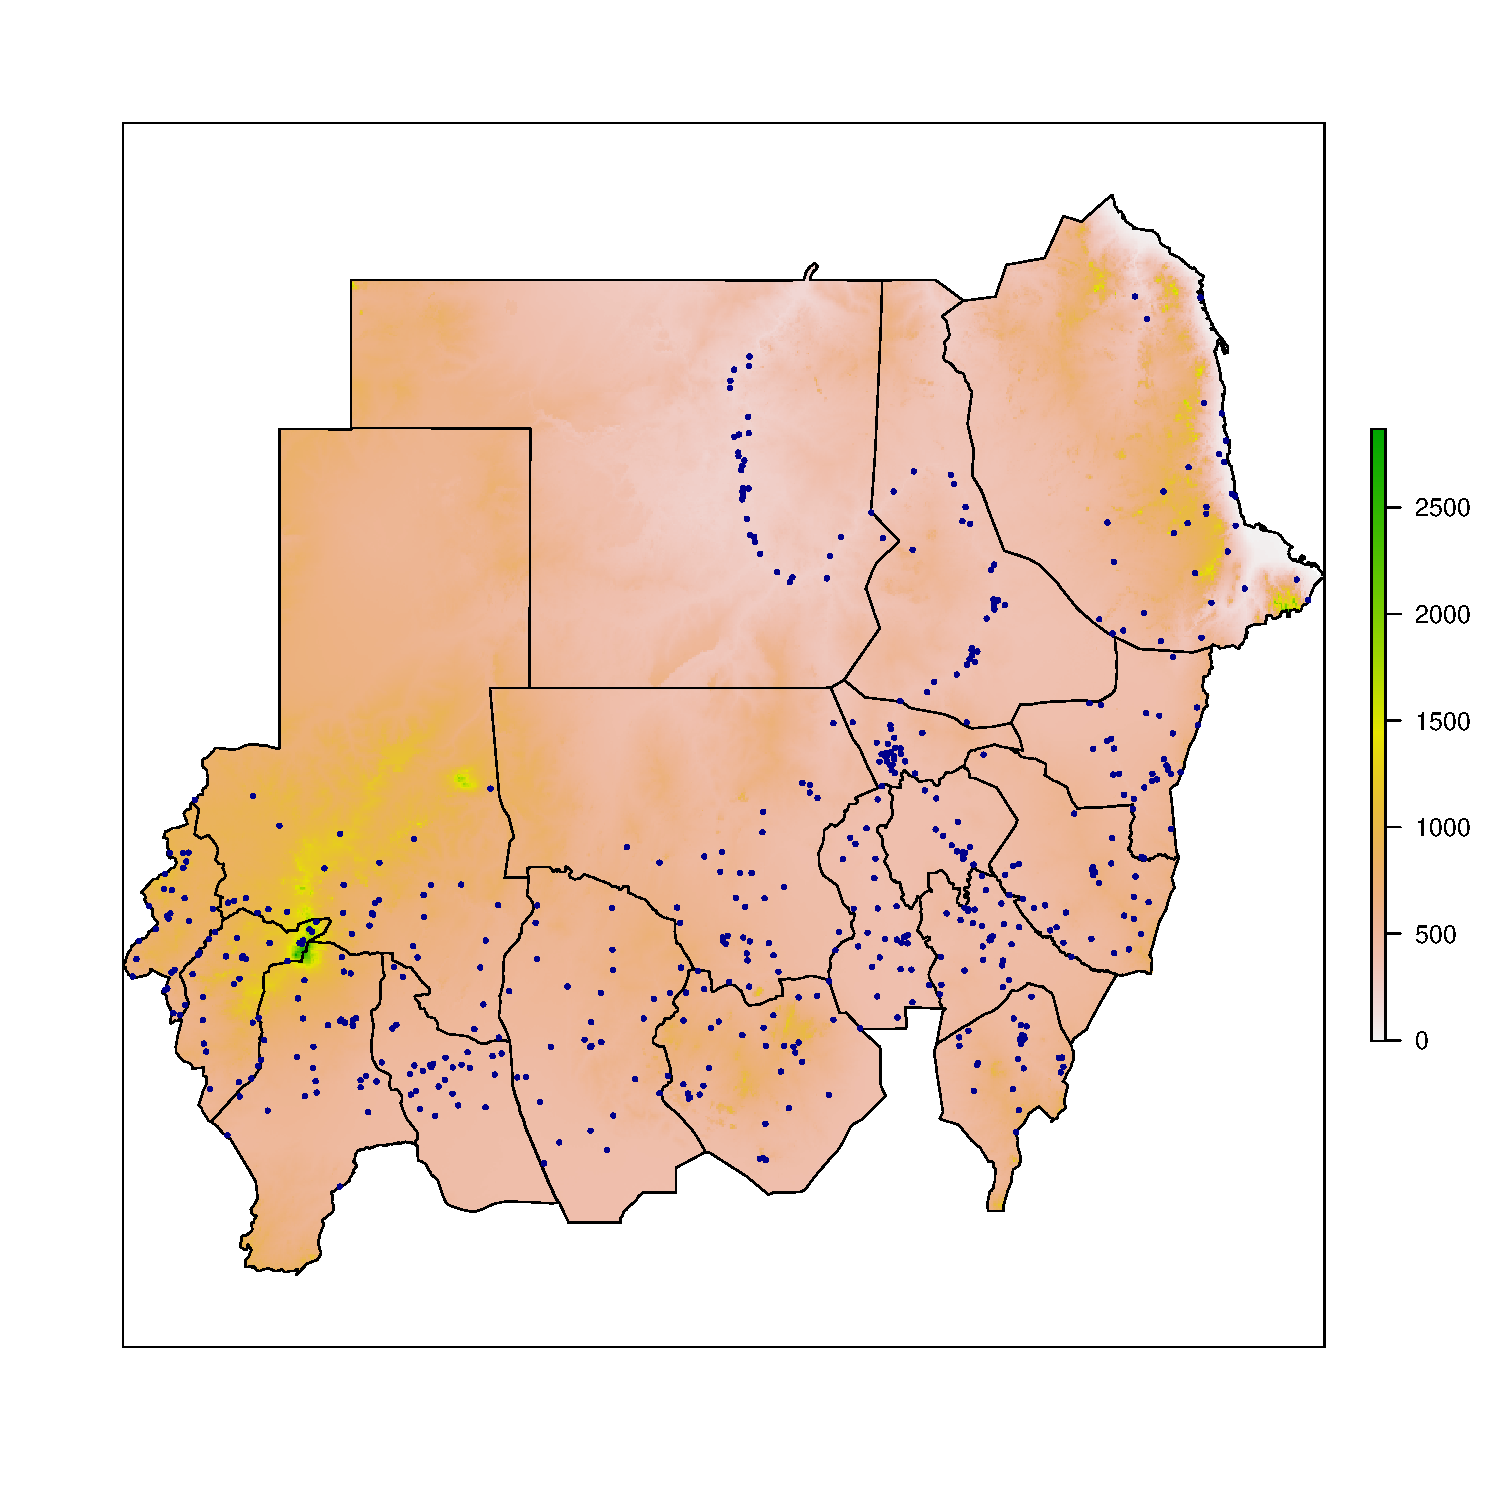
\includegraphics{sudanMNindicators_files/figure-latex/elevation1-1} 

}

\caption{Shuttle Radar Topography Mission (SRTM) 90m Digital Elevation Model (DEM) for Sudan overlaid with the Sudan National Micronutrient survey primary sampling unit locations}\label{fig:elevation1}
\end{figure}

With this data, we are able to extract elevation data for each of the PSUs in the Sudan Micronutrient Survey dataset.

\newpage

\begin{table}[H]

\caption{\label{tab:elevation2}Sudan National Micronutrient Survey dataset with altitude extracted from SRTM 90m DEM}
\centering
\begin{tabular}[t]{rrrrlr}
\toprule
\textbf{psu} & \textbf{state} & \textbf{locality} & \textbf{sex} & \textbf{hb} & \textbf{altitude}\\
\midrule
\rowcolor{gray!6}  45 & 16 & 164 & 2 & 11.6 & \vphantom{1} 978\\
45 & 16 & 164 & 2 & 13.9 & 978\\
\rowcolor{gray!6}  45 & 16 & 164 & 2 & 12.4 & \vphantom{2} 978\\
45 & 16 & 164 & 2 & 13.1 & 978\\
\rowcolor{gray!6}  45 & 16 & 164 & 2 & 13.2 & 978\\
\addlinespace
45 & 16 & 164 & 2 & 10.3 & 978\\
\rowcolor{gray!6}  45 & 16 & 164 & 2 & 12.4 & \vphantom{1} 978\\
45 & 16 & 164 & 1 & 8.8000000000000007 & 978\\
\rowcolor{gray!6}  45 & 16 & 164 & 2 & 11.8 & \vphantom{1} 978\\
45 & 16 & 164 & 1 & 8.1 & 978\\
\addlinespace
\rowcolor{gray!6}  45 & 16 & 164 & 2 & 12.4 & \vphantom{2} 978\\
45 & 16 & 164 & 2 & 9.1 & 978\\
\rowcolor{gray!6}  45 & 16 & 164 & 2 & 13.3 & 978\\
45 & 16 & 164 & 1 & 9.8000000000000007 & 978\\
\rowcolor{gray!6}  45 & 16 & 164 & 2 & 10.4 & 978\\
\addlinespace
45 & 16 & 164 & 2 & 13 & \vphantom{1} 978\\
\rowcolor{gray!6}  45 & 16 & 164 & 2 & 11.8 & \vphantom{1} 978\\
45 & 16 & 164 & 2 & 13 & \vphantom{1} 978\\
\rowcolor{gray!6}  45 & 16 & 164 & 2 & 8.5 & 978\\
45 & 16 & 164 & 2 & 8.6 & 978\\
\addlinespace
\rowcolor{gray!6}  45 & 16 & 164 & 2 & 11.4 & 978\\
45 & 16 & 164 & 2 & 12.6 & 978\\
\rowcolor{gray!6}  45 & 16 & 164 & 2 & 8.9 & 978\\
45 & 16 & 164 & 2 & 14.2 & 978\\
\rowcolor{gray!6}  45 & 16 & 164 & 1 & 10.5 & 978\\
\addlinespace
45 & 16 & 164 & 2 & 11.9 & 978\\
\rowcolor{gray!6}  45 & 16 & 164 & 2 & 11.6 & \vphantom{1} 978\\
45 & 16 & 164 & 2 & 10.7 & 978\\
\rowcolor{gray!6}  45 & 16 & 164 & 2 & 10.8 & 978\\
53 & 16 & 164 & 1 & 10.6 & 874\\
\addlinespace
\rowcolor{gray!6}  53 & 16 & 164 & 2 & 10 & 874\\
53 & 16 & 164 & NA & NA & 874\\
\rowcolor{gray!6}  53 & 16 & 164 & 1 & 11.8 & 874\\
53 & 16 & 164 & 2 & NA & 874\\
\rowcolor{gray!6}  53 & 16 & 164 & 2 & 12.4 & 874\\
\addlinespace
53 & 16 & 164 & 1 & 7.9 & 874\\
\rowcolor{gray!6}  53 & 16 & 164 & 1 & 8.4 & 874\\
53 & 16 & 164 & 2 & 11.7 & 874\\
\rowcolor{gray!6}  53 & 16 & 164 & 2 & 10.6 & 874\\
53 & 16 & 164 & 2 & 12.5 & 874\\
\bottomrule
\end{tabular}
\end{table}

Adjustments to measured Hb based on altitude will be done based on the following \citep{WorldHealthOrganization:2011ut}:

\begin{table}[H]

\caption{\label{tab:hb2}Altitude adjustments to measured haemoglobin concentrations}
\centering
\begin{tabular}[t]{lr}
\toprule
\textbf{\makecell[c]{Altitude\\(metres above\\sea level)}} & \textbf{\makecell[c]{Measured\\haemoglobin\\adjustment\\(g/L)}}\\
\midrule
\rowcolor{gray!6}  < 1000 & 0\\
1000 & -2\\
\rowcolor{gray!6}  1500 & -5\\
2000 & -8\\
\rowcolor{gray!6}  2500 & -13\\
\addlinespace
3000 & -19\\
\rowcolor{gray!6}  3500 & -27\\
4000 & -35\\
\rowcolor{gray!6}  4500 & -45\\
\bottomrule
\end{tabular}
\end{table}

\hypertarget{serum-ferritin-and-c-reactive-protein}{%
\subsection{Serum ferritin and c-reactive protein}\label{serum-ferritin-and-c-reactive-protein}}

Normal serum ferritin levels range from 12 µg/L to 150 µg/L. Following are the cut-offs for serum ferritin concentration that indicate either iron depletion or iron overload \citep{WorldHealthOrganization:2007tx, Gorstein:2007wn, Wegmuller:2020bw, WorldHealthOrganization:2011ue}.

\begin{table}[H]

\caption{\label{tab:ferritin}Relative extent of iron stores on the basis of serum ferritin concentration (µg/L)}
\centering
\resizebox{\linewidth}{!}{
\begin{tabular}[t]{>{\bfseries}lllll}
\toprule
\multicolumn{1}{c}{\textbf{ }} & \multicolumn{4}{c}{\textbf{Serum ferritin (µg/L)}} \\
\cmidrule(l{3pt}r{3pt}){2-5}
\multicolumn{1}{c}{\textbf{ }} & \multicolumn{2}{c}{\textbf{Less than 5 years}} & \multicolumn{2}{c}{\textbf{5 years or older}} \\
\cmidrule(l{3pt}r{3pt}){2-3} \cmidrule(l{3pt}r{3pt}){4-5}
\multicolumn{1}{c}{\textbf{}} & \multicolumn{1}{c}{\textbf{Male}} & \multicolumn{1}{c}{\textbf{Female}} & \multicolumn{1}{c}{\textbf{Male}} & \multicolumn{1}{c}{\textbf{Female}}\\
\midrule
\rowcolor{gray!6}  Depleted iron stores & < 12 & < 12 & < 15 & < 15\\
Depleted iron stores in the presence of infection & < 30 & < 30 & - & -\\
\rowcolor{gray!6}  Severe risk of iron overload (adults) & - & - & > 200 & > 150\\
\bottomrule
\end{tabular}}
\end{table}

Serum ferritin will be used to assess iron deficiency for children less than 5 and for any other individual above 5 years old. For children less than 5 years old, a cut-off for serum ferritin value of \textless{} 12 \(\mu/L\) indicates iron deficiency while for those older than 5 years old, a cut-off of \textless{} 15 \(\mu/L\) is used.

However, it has been recommended that serum ferritin values be adjusted based on inflammation status ideally using both of the acute phase proteins - C-reactive protein (CRP) and \(\alpha_1\)-acid glycoprotein (AGP) to yield the most unbiased estimates of iron deficiency. However, the Sudan Micronutrient Survey only assessed CRP in the samples. The recommended adjustments when only one of the active phase proteins is available is to use an appropriate multiplier to the serum ferritin value depending on inflammation status of the respondent as described below:

\begin{table}[H]

\caption{\label{tab:inflammation}Cut-offs to determine inflammation}
\centering
\begin{tabular}[t]{ll}
\toprule
\textbf{Active Phase Protein} & \textbf{Cut-off}\\
\midrule
\rowcolor{gray!6}  CRP & > 5 mg/L\\
AGP & > 1 g/L\\
\bottomrule
\end{tabular}
\end{table}

If a respondent is classified as being in an active inflammation process, then serum ferritin is adjusted accordingly. If inflammation is assessed using CRP only, the serum ferritin is adjusted by 0.65 \citep{Thurnham:2010he}.

\hypertarget{calcium}{%
\subsection{Calcium}\label{calcium}}

The range of normal values for serum calcium is age-dependent as shown below \citep{Lietman:2010iu}:

\begin{table}[H]

\caption{\label{tab:calcium}Representative normal values for age for concentration of serum total calcium}
\centering
\begin{tabular}[t]{lll}
\toprule
\textbf{\makecell[c]{Target\\Group}} & \textbf{Age} & \textbf{\makecell[c]{Serum\\total calcium\\(mg/dL)}}\\
\midrule
\rowcolor{gray!6}   & 0-3 months & 8.8 - 11.3\\
\cmidrule{2-3}
\multirow[t]{-2}{*}{\raggedright\arraybackslash Infants} & 1-5 years & 9.4 - 10.8\\
\cmidrule{1-3}
\rowcolor{gray!6}  Children & 6-12 years & 9.4 - 10.3\\
\cmidrule{1-3}
 & 20 years & 9.1 - 10.2\\
\cmidrule{2-3}
\rowcolor{gray!6}   & 50 years & 8.9 - 10.0\\
\cmidrule{2-3}
\multirow[t]{-3}{*}{\raggedright\arraybackslash Men} & 70 years & 8.8 - 9.9\\
\cmidrule{1-3}
\rowcolor{gray!6}   & 20 years & 8.8 - 10.0\\
\cmidrule{2-3}
 & 50 years & 8.8 - 10.0\\
\cmidrule{2-3}
\rowcolor{gray!6}  \multirow[t]{-3}{*}{\raggedright\arraybackslash Women} & 70 years & 8.8 - 10.0\\
\bottomrule
\end{tabular}
\end{table}

We propose to use these normal ranges by age to determine whether a specific respondent group is hypocalcemic or below the normal range for their age or hypercalcemic or above the normal range for their age.

\hypertarget{iodine}{%
\subsection{Iodine}\label{iodine}}

Currently, cut-offs for urinary iodine are available for school-age children and older (6 years and older), pregnant women, and for lactating women and children aged less than 2 years.

Following are the various criteria for assessing iodine status in school-age children and older \citep{WorldHealthOrganization:2013wl}:

\begin{table}[H]

\caption{\label{tab:iodine1}Epidemiologic criteria for assessing iodine nutrition based on median urinary iodine concentration in school-age children and older}
\centering
\begin{tabular}[t]{ll>{\raggedright\arraybackslash}p{8cm}}
\toprule
\textbf{\makecell[c]{Median urinary\\iodine (µg/L)}} & \textbf{Iodine intake} & \textbf{Iodine status}\\
\midrule
\rowcolor{gray!6}  < 20 & Insufficient & Severe iodine deficiency\\
20 - 49 & Insufficient & Moderate iodine deficiency\\
\rowcolor{gray!6}  50 - 99 & Insufficient & Mild iodine deficiency\\
100 - 199 & Adequate & Adequate iodine nutrition\\
\rowcolor{gray!6}  200 - 299 & Above requirements & May pose a slight risk of more than adequate iodine intake in these populations\\
\addlinespace
≥ 300 & Excessive & Risk of adverse health consequences (iodine-induced hyperthyroidism, autoimmune thyroid disease)\\
\bottomrule
\end{tabular}
\end{table}

Following are the various criteria for assessing iodine status in pregnant women, lactating women and children aged less than 2 years \citep{WorldHealthOrganization:2013wl}:

\begin{table}[H]

\caption{\label{tab:iodine2}Epidemiologic criteria for assessing iodine nutrition based on median urinary iodine concentration in pregnant women, lactating women, and children aged less than 2 years}
\centering
\begin{tabular}[t]{ll}
\toprule
\textbf{Median urinary iodine (g/L)} & \textbf{Iodine intake}\\
\midrule
\rowcolor{gray!6}  \addlinespace[0.3em]
\multicolumn{2}{l}{\textbf{Pregnant women}}\\
\hspace{1em}< 150 & Insufficient\\
\hspace{1em}150 - 249 & Adequate\\
\rowcolor{gray!6}  \hspace{1em}250 - 499 & Above requirements\\
\hspace{1em}500 or more & Excessive\\
\rowcolor{gray!6}  \addlinespace[0.3em]
\multicolumn{2}{l}{\textbf{Lactating women and children aged less than 2 years}}\\
\hspace{1em}< 100 & Insufficient\\
\hspace{1em}100 or more & Adequate\\
\bottomrule
\end{tabular}
\end{table}

\hypertarget{micronutrient-indicators}{%
\section{Micronutrient indicators}\label{micronutrient-indicators}}

Given the biomarkers variables described above, we propose the following indicator sets.

\hypertarget{anaemia-prevalence-indicators}{%
\subsection{Anaemia prevalence indicators}\label{anaemia-prevalence-indicators}}

The anaemia indicators are:

\begin{table}[H]

\caption{\label{tab:anaemia1}Anaemia indicators}
\centering
\begin{tabular}[t]{ll}
\toprule
\textbf{} & \textbf{}\\
\midrule
\rowcolor{gray!6}  AN1 & Mild anaemia in children 6-59 months\\
AN1 & Mild anaemia in non-pregnant carers\\
\rowcolor{gray!6}  AN1 & Mild anaemia in pregnant carers\\
AN2 & Moderate anaemia in children 6-59 months\\
\rowcolor{gray!6}  AN2 & Moderate anaemia in non-pregnant carers\\
\addlinespace
AN2 & Moderate anaemia in pregnant carers\\
\rowcolor{gray!6}  AN3 & Severe anaemia in children 6-59 months\\
AN3 & Severe anaemia in non-pregnant carers\\
\rowcolor{gray!6}  AN3 & Severe anaemia in pregnant carers\\
\bottomrule
\end{tabular}
\end{table}

The anaemia indicators are calculated using data on \textbf{AGE}, \textbf{SEX}, \textbf{PREGNANCY} status and \textbf{HB} measurement (in g/L) of the respondent and on the \textbf{ALTITUDE} (in metres) of the location where the respondent resides.

\hypertarget{an1-mild-anaemia}{%
\subsubsection{AN1: Mild anaemia}\label{an1-mild-anaemia}}

Indicator \textbf{AN1} is TRUE if either\ldots{}

\begin{itemize}
\item
  \{(\textbf{AGE} of respondent is between 6-59 months old) \textbf{\emph{or}} (\textbf{AGE} of respondent is between 15 and 49 years old \textbf{\emph{and}} \textbf{SEX} is \textbf{FEMALE} \textbf{\emph{and}} \textbf{PREGNANT})\} \textbf{\emph{and}}

  \begin{itemize}
  \item
    \textbf{ALTITUDE} is \textbf{\emph{\textless{}}} 1000 metres \textbf{\emph{and}} \textbf{HB} is \textbf{\emph{\(\geq\)}} 100 g/L \textbf{\emph{and}} \textbf{HB}
    is \textbf{\emph{\(\leq\)}} 109 g/L; \textbf{\emph{or}},
  \item
    \textbf{ALTITUDE} is \textbf{\emph{\(\geq\)}} 1000 metres \textbf{\emph{and}} \textbf{ALTITUDE} is \textbf{\emph{\textless{}}} 1500 metres \textbf{\emph{and}} \textbf{HB} is \textbf{\emph{\(\geq\)}} 102 g/L \textbf{\emph{and}} \textbf{HB} is \textbf{\emph{\(\leq\)}} 111 g/L; \textbf{\emph{or}},
  \item
    \textbf{ALTITUDE} is \textbf{\emph{\(\geq\)}} 1500 metres \textbf{\emph{and}} \textbf{ALTITUDE} is \textbf{\emph{\textless{}}} 2000 metres \textbf{\emph{and}} \textbf{HB} is \textbf{\emph{\(\geq\)}} 105 g/L \textbf{\emph{and}} \textbf{HB} is \textbf{\emph{\(\leq\)}} 114 g/L; \textbf{\emph{or}},
  \item
    \textbf{ALTITUDE} is \textbf{\emph{\(\geq\)}} 2000 metres \textbf{\emph{and}} \textbf{ALTITUDE} is \textbf{\emph{\textless{}}} 2500 metres \textbf{\emph{and}} \textbf{HB} is \textbf{\emph{\(\geq\)}} 108 g/L \textbf{\emph{and}} \textbf{HB} is \textbf{\emph{\(\leq\)}} 117 g/L; \textbf{\emph{or}},
  \item
    \textbf{ALTITUDE} is \textbf{\emph{\(\geq\)}} 2500 metres \textbf{\emph{and}} \textbf{ALTITUDE} is \textbf{\emph{\textless{}}} 3000 metres \textbf{\emph{and}} \textbf{HB} is \textbf{\emph{\(\geq\)}} 113 g/L \textbf{\emph{and}} \textbf{HB} is \textbf{\emph{\(\leq\)}} 122 g/L; \textbf{\emph{or}},
  \item
    \textbf{ALTITUDE} is \textbf{\emph{\(\geq\)}} 3000 metres \textbf{\emph{and}} \textbf{ALTITUDE} is \textbf{\emph{\textless{}}} 3500 metres \textbf{\emph{and}} \textbf{HB} is \textbf{\emph{\(\geq\)}} 119 g/L \textbf{\emph{and}} \textbf{HB} is \textbf{\emph{\(\leq\)}} 128 g/L; \textbf{\emph{or}},
  \item
    \textbf{ALTITUDE} is \textbf{\emph{\(\geq\)}} 3500 metres \textbf{\emph{and}} \textbf{ALTITUDE} is \textbf{\emph{\textless{}}} 4000 metres \textbf{\emph{and}} \textbf{HB} is \textbf{\emph{\(\geq\)}} 127 g/L \textbf{\emph{and}} \textbf{HB} is \textbf{\emph{\(\leq\)}} 136 g/L; \textbf{\emph{or}},
  \item
    \textbf{ALTITUDE} is \textbf{\emph{\(\geq\)}} 4000 metres \textbf{\emph{and}} \textbf{ALTITUDE} is \textbf{\emph{\textless{}}} 4500 metres \textbf{\emph{and}} \textbf{HB} is \textbf{\emph{\(\geq\)}} 135 g/L \textbf{\emph{and}} \textbf{HB} is \textbf{\emph{\(\leq\)}} 144 g/L; \textbf{\emph{or}},
  \item
    \textbf{ALTITUDE} is \textbf{\emph{=}} 4500 metres \textbf{\emph{and}} \textbf{HB} is \textbf{\emph{\(\geq\)}} 145 g/L \textbf{\emph{and}} \textbf{HB} is \textbf{\emph{\(\leq\)}} 154 g/L; \textbf{\emph{or}},
  \end{itemize}
\item
  \textbf{AGE} of respondent is between 15 and 49 years \textbf{\emph{and}} \textbf{SEX} is \textbf{\emph{FEMALE}} \textbf{\emph{and}} \textbf{NOT PREGNANT} \textbf{\emph{and}}

  \begin{itemize}
  \item
    \textbf{ALTITUDE} is \textbf{\emph{\textless{}}} 1000 metres \textbf{\emph{and}} \textbf{HB} is \textbf{\emph{\(\geq\)}} 110 g/L \textbf{\emph{and}} \textbf{HB} is \textbf{\emph{\(\leq\)}} 119 g/L; \textbf{\emph{or}},
  \item
    \textbf{ALTITUDE} is \textbf{\emph{\(\geq\)}} 1000 metres \textbf{\emph{and}} \textbf{ALTITUDE} is \textbf{\emph{\textless{}}} 1500 metres \textbf{\emph{and}} \textbf{HB} is \textbf{\emph{\(\geq\)}} 112 g/L \textbf{\emph{and}} \textbf{HB} is \textbf{\emph{\(\leq\)}} 121 g/L; \textbf{\emph{or}},
  \item
    \textbf{ALTITUDE} is \textbf{\emph{\(\geq\)}} 1500 metres \textbf{\emph{and}} \textbf{ALTITUDE} is \textbf{\emph{\textless{}}} 2000 metres \textbf{\emph{and}} \textbf{HB} is \textbf{\emph{\(\geq\)}} 115 g/L \textbf{\emph{and}} \textbf{HB} is \textbf{\emph{\(\leq\)}} 124 g/L; \textbf{\emph{or}},
  \item
    \textbf{ALTITUDE} is \textbf{\emph{\(\geq\)}} 2000 metres \textbf{\emph{and}} \textbf{ALTITUDE} is \textbf{\emph{\textless{}}} 2500 metres \textbf{\emph{and}} \textbf{HB} is \textbf{\emph{\(\geq\)}} 118 g/L \textbf{\emph{and}} \textbf{HB} is \textbf{\emph{\(\leq\)}} 127 g/L; \textbf{\emph{or}},
  \item
    \textbf{ALTITUDE} is \textbf{\emph{\(\geq\)}} 2500 metres \textbf{\emph{and}} \textbf{ALTITUDE} is \textbf{\emph{\textless{}}} 3000 metres \textbf{\emph{and}} \textbf{HB} is \textbf{\emph{\(\geq\)}} 123 g/L \textbf{\emph{and}} \textbf{HB} is \textbf{\emph{\(\leq\)}} 132 g/L; \textbf{\emph{or}},
  \item
    \textbf{ALTITUDE} is \textbf{\emph{\(\geq\)}} 3000 metres \textbf{\emph{and}} \textbf{ALTITUDE} is \textbf{\emph{\textless{}}} 3500 metres \textbf{\emph{and}} \textbf{HB} is \textbf{\emph{\(\geq\)}} 129 g/L \textbf{\emph{and}} \textbf{HB} is \textbf{\emph{\(\leq\)}} 138 g/L; \textbf{\emph{or}},
  \item
    \textbf{ALTITUDE} is \textbf{\emph{\(\geq\)}} 3500 metres \textbf{\emph{and}} \textbf{ALTITUDE} is \textbf{\emph{\textless{}}} 4000 metres \textbf{\emph{and}} \textbf{HB} is \textbf{\emph{\(\geq\)}} 137 g/L \textbf{\emph{and}} \textbf{HB} is \textbf{\emph{\(\leq\)}} 146 g/L; \textbf{\emph{or}},
  \item
    \textbf{ALTITUDE} is \textbf{\emph{\(\geq\)}} 4000 metres \textbf{\emph{and}} \textbf{ALTITUDE} is \textbf{\emph{\textless{}}} 4500 metres \textbf{\emph{and}} \textbf{HB} is \textbf{\emph{\(\geq\)}} 145 g/L \textbf{\emph{and}} \textbf{HB} is \textbf{\emph{\(\leq\)}} 154 g/L; \textbf{\emph{or}},
  \item
    \textbf{ALTITUDE} is \textbf{\emph{=}} 4500 metres \textbf{\emph{and}} \textbf{HB} is \textbf{\emph{\(\geq\)}} 155 g/L and \textbf{HB} is \textbf{\emph{\(\leq\)}} 164 g/L.
  \end{itemize}
\end{itemize}

\hypertarget{an2-moderate-anaemia}{%
\subsubsection{AN2: Moderate anaemia}\label{an2-moderate-anaemia}}

Indicator \textbf{AN2} is TRUE if either\ldots{}

\begin{itemize}
\item
  \{(\textbf{AGE} of respondent is between 6-59 months old) \textbf{\emph{or}} (\textbf{AGE} of respondent is between 15 and 49 years old \textbf{\emph{and}} \textbf{SEX} is \textbf{FEMALE} \textbf{\emph{and}} \textbf{PREGNANT})\} \textbf{\emph{and}}

  \begin{itemize}
  \item
    \textbf{ALTITUDE} is \textbf{\emph{\textless{}}} 1000 metres \textbf{\emph{and}} \textbf{HB} is \textbf{\emph{\(\geq\)}} 70 g/L \textbf{\emph{and}} \textbf{HB}
    is \textbf{\emph{\(\leq\)}} 99 g/L; \textbf{\emph{or}},
  \item
    \textbf{ALTITUDE} is \textbf{\emph{\(\geq\)}} 1000 metres \textbf{\emph{and}} \textbf{ALTITUDE} is \textbf{\emph{\textless{}}} 1500 metres \textbf{\emph{and}} \textbf{HB} is \textbf{\emph{\(\geq\)}} 72 g/L \textbf{\emph{and}} \textbf{HB} is \textbf{\emph{\(\leq\)}} 101 g/L; \textbf{\emph{or}},
  \item
    \textbf{ALTITUDE} is \textbf{\emph{\(\geq\)}} 1500 metres \textbf{\emph{and}} \textbf{ALTITUDE} is \textbf{\emph{\textless{}}} 2000 metres \textbf{\emph{and}} \textbf{HB} is \textbf{\emph{\(\geq\)}} 75 g/L \textbf{\emph{and}} \textbf{HB} is \textbf{\emph{\(\leq\)}} 104 g/L; \textbf{\emph{or}},
  \item
    \textbf{ALTITUDE} is \textbf{\emph{\(\geq\)}} 2000 metres \textbf{\emph{and}} \textbf{ALTITUDE} is \textbf{\emph{\textless{}}} 2500 metres \textbf{\emph{and}} \textbf{HB} is \textbf{\emph{\(\geq\)}} 78 g/L \textbf{\emph{and}} \textbf{HB} is \textbf{\emph{\(\leq\)}} 107 g/L; \textbf{\emph{or}},
  \item
    \textbf{ALTITUDE} is \textbf{\emph{\(\geq\)}} 2500 metres \textbf{\emph{and}} \textbf{ALTITUDE} is \textbf{\emph{\textless{}}} 3000 metres \textbf{\emph{and}} \textbf{HB} is \textbf{\emph{\(\geq\)}} 83 g/L \textbf{\emph{and}} \textbf{HB} is \textbf{\emph{\(\leq\)}} 112 g/L; \textbf{\emph{or}},
  \item
    \textbf{ALTITUDE} is \textbf{\emph{\(\geq\)}} 3000 metres \textbf{\emph{and}} \textbf{ALTITUDE} is \textbf{\emph{\textless{}}} 3500 metres \textbf{\emph{and}} \textbf{HB} is \textbf{\emph{\(\geq\)}} 89 g/L \textbf{\emph{and}} \textbf{HB} is \textbf{\emph{\(\leq\)}} 118 g/L; \textbf{\emph{or}},
  \item
    \textbf{ALTITUDE} is \textbf{\emph{\(\geq\)}} 3500 metres \textbf{\emph{and}} \textbf{ALTITUDE} is \textbf{\emph{\textless{}}} 4000 metres \textbf{\emph{and}} \textbf{HB} is \textbf{\emph{\(\geq\)}} 97 g/L \textbf{\emph{and}} \textbf{HB} is \textbf{\emph{\(\leq\)}} 126 g/L; \textbf{\emph{or}},
  \item
    \textbf{ALTITUDE} is \textbf{\emph{\(\geq\)}} 4000 metres \textbf{\emph{and}} \textbf{ALTITUDE} is \textbf{\emph{\textless{}}} 4500 metres \textbf{\emph{and}} \textbf{HB} is \textbf{\emph{\(\geq\)}} 105 g/L \textbf{\emph{and}} \textbf{HB} is \textbf{\emph{\(\leq\)}} 134 g/L; \textbf{\emph{or}},
  \item
    \textbf{ALTITUDE} is \textbf{\emph{=}} 4500 metres \textbf{\emph{and}} \textbf{HB} is \textbf{\emph{\(\geq\)}} 115 g/L \textbf{\emph{and}} \textbf{\emph{\(\leq\)}} 144 g/L; \textbf{\emph{or}},
  \end{itemize}
\item
  \textbf{AGE} of respondent is between 15 and 49 years \textbf{\emph{and}} \textbf{SEX} is \textbf{\emph{FEMALE}} \textbf{\emph{and}} \textbf{NOT PREGNANT} \textbf{\emph{and}}

  \begin{itemize}
  \item
    \textbf{ALTITUDE} is \textbf{\emph{\textless{}}} 1000 metres \textbf{\emph{and}} \textbf{HB} is \textbf{\emph{\(\geq\)}} 80 g/L \textbf{\emph{and}} \textbf{HB} is \textbf{\emph{\(\leq\)}} 109 g/L; \textbf{\emph{or}},
  \item
    \textbf{ALTITUDE} is \textbf{\emph{\(\geq\)}} 1000 metres \textbf{\emph{and}} \textbf{ALTITUDE} is \textbf{\emph{\textless{}}} 1500 metres \textbf{\emph{and}} \textbf{HB} is \textbf{\emph{\(\geq\)}} 82 g/L \textbf{\emph{and}} \textbf{HB} is \textbf{\emph{\(\leq\)}} 111 g/L; \textbf{\emph{or}},
  \item
    \textbf{ALTITUDE} is \textbf{\emph{\(\geq\)}} 1500 metres \textbf{\emph{and}} \textbf{ALTITUDE} is \textbf{\emph{\textless{}}} 2000 metres \textbf{\emph{and}} \textbf{HB} is \textbf{\emph{\(\geq\)}} 85 g/L \textbf{\emph{and}} \textbf{HB} is \textbf{\emph{\(\leq\)}} 114 g/L; \textbf{\emph{or}},
  \item
    \textbf{ALTITUDE} is \textbf{\emph{\(\geq\)}} 2000 metres \textbf{\emph{and}} \textbf{ALTITUDE} is \textbf{\emph{\textless{}}} 2500 metres \textbf{\emph{and}} \textbf{HB} is \textbf{\emph{\(\geq\)}} 88 g/L \textbf{\emph{and}} \textbf{HB} is \textbf{\emph{\(\leq\)}} 117 g/L; \textbf{\emph{or}},
  \item
    \textbf{ALTITUDE} is \textbf{\emph{\(\geq\)}} 2500 metres \textbf{\emph{and}} \textbf{ALTITUDE} is \textbf{\emph{\textless{}}} 3000 metres \textbf{\emph{and}} \textbf{HB} is \textbf{\emph{\(\geq\)}} 93 g/L \textbf{\emph{and}} \textbf{HB} is \textbf{\emph{\(\leq\)}} 122 g/L; \textbf{\emph{or}},
  \item
    \textbf{ALTITUDE} is \textbf{\emph{\(\geq\)}} 3000 metres \textbf{\emph{and}} \textbf{ALTITUDE} is \textbf{\emph{\textless{}}} 3500 metres \textbf{\emph{and}} \textbf{HB} is \textbf{\emph{\(\geq\)}} 99 g/L \textbf{\emph{and}} \textbf{HB} is \textbf{\emph{\(\leq\)}} 128 g/L; \textbf{\emph{or}},
  \item
    \textbf{ALTITUDE} is \textbf{\emph{\(\geq\)}} 3500 metres \textbf{\emph{and}} \textbf{ALTITUDE} is \textbf{\emph{\textless{}}} 4000 metres \textbf{\emph{and}} \textbf{HB} is \textbf{\emph{\(\geq\)}} 107 g/L \textbf{\emph{and}} \textbf{HB} is \textbf{\emph{\(\leq\)}} 136 g/L; \textbf{\emph{or}},
  \item
    \textbf{ALTITUDE} is \textbf{\emph{\(\geq\)}} 4000 metres \textbf{\emph{and}} \textbf{ALTITUDE} is \textbf{\emph{\textless{}}} 4500 metres \textbf{\emph{and}} \textbf{HB} is \textbf{\emph{\(\geq\)}} 115 g/L \textbf{\emph{and}} \textbf{HB} is \textbf{\emph{\(\leq\)}} 144 g/L; \textbf{\emph{or}},
  \item
    \textbf{ALTITUDE} is \textbf{\emph{=}} 4500 metres \textbf{\emph{and}} \textbf{HB} is \textbf{\emph{\(\geq\)}} 125 g/L and \textbf{HB} is \textbf{\emph{\(\leq\)}} 154 g/L.
  \end{itemize}
\end{itemize}

\hypertarget{an3-severe-anaemia}{%
\subsubsection{AN3: Severe anaemia}\label{an3-severe-anaemia}}

Indicator \textbf{AN3} is TRUE if either\ldots{}

\begin{itemize}
\item
  \{(\textbf{AGE} of respondent is between 6-59 months old) \textbf{\emph{or}} (\textbf{AGE} of respondent is between 15 and 49 years old \textbf{\emph{and}} \textbf{SEX} is \textbf{FEMALE} \textbf{\emph{and}} \textbf{PREGNANT})\} \textbf{\emph{and}}

  \begin{itemize}
  \item
    \textbf{ALTITUDE} is \textbf{\emph{\textless{}}} 1000 metres \textbf{\emph{and}} \textbf{HB} is \textbf{\emph{\textless{}}} 70 g/L; \textbf{\emph{or}},
  \item
    \textbf{ALTITUDE} is \textbf{\emph{\(\geq\)}} 1000 metres \textbf{\emph{and}} \textbf{ALTITUDE} is \textbf{\emph{\textless{}}} 1500 metres \textbf{\emph{and}} \textbf{HB} is \textbf{\emph{\textless{}}} 72 g/L; \textbf{\emph{or}},
  \item
    \textbf{ALTITUDE} is \textbf{\emph{\(\geq\)}} 1500 metres \textbf{\emph{and}} \textbf{ALTITUDE} is \textbf{\emph{\textless{}}} 2000 metres \textbf{\emph{and}} \textbf{HB} is \textbf{\emph{\textless{}}} 75 g/L; \textbf{\emph{or}},
  \item
    \textbf{ALTITUDE} is \textbf{\emph{\(\geq\)}} 2000 metres \textbf{\emph{and}} \textbf{ALTITUDE} is \textbf{\emph{\textless{}}} 2500 metres \textbf{\emph{and}} \textbf{HB} is \textbf{\emph{\textless{}}} 78 g/L; \textbf{\emph{or}},
  \item
    \textbf{ALTITUDE} is \textbf{\emph{\(\geq\)}} 2500 metres \textbf{\emph{and}} \textbf{ALTITUDE} is \textbf{\emph{\textless{}}} 3000 metres \textbf{\emph{and}} \textbf{HB} is \textbf{\emph{\textless{}}} 83 g/L; \textbf{\emph{or}},
  \item
    \textbf{ALTITUDE} is \textbf{\emph{\(\geq\)}} 3000 metres \textbf{\emph{and}} \textbf{ALTITUDE} is \textbf{\emph{\textless{}}} 3500 metres \textbf{\emph{and}} \textbf{HB} is \textbf{\emph{\textless{}}} 89 g/L; \textbf{\emph{or}},
  \item
    \textbf{ALTITUDE} is \textbf{\emph{\(\geq\)}} 3500 metres \textbf{\emph{and}} \textbf{ALTITUDE} is \textbf{\emph{\textless{}}} 4000 metres \textbf{\emph{and}} \textbf{HB} is \textbf{\emph{\textless{}}} 97 g/L; \textbf{\emph{or}},
  \item
    \textbf{ALTITUDE} is \textbf{\emph{\(\geq\)}} 4000 metres \textbf{\emph{and}} \textbf{ALTITUDE} is \textbf{\emph{\textless{}}} 4500 metres \textbf{\emph{and}} \textbf{HB} is \textbf{\emph{\textless{}}} 105 g/L; \textbf{\emph{or}},
  \item
    \textbf{ALTITUDE} is \textbf{\emph{=}} 4500 metres \textbf{\emph{and}} \textbf{HB} is \textbf{\emph{\textless{}}} 115 g/L; \textbf{\emph{or}},
  \end{itemize}
\item
  \textbf{AGE} of respondent is between 15 and 49 years \textbf{\emph{and}} \textbf{SEX} is \textbf{\emph{FEMALE}} \textbf{\emph{and}} \textbf{NOT PREGNANT} \textbf{\emph{and}}

  \begin{itemize}
  \item
    \textbf{ALTITUDE} is \textbf{\emph{\textless{}}} 1000 metres \textbf{\emph{and}} \textbf{HB} is \textbf{\emph{\textless{}}} 80 g/L; \textbf{\emph{or}},
  \item
    \textbf{ALTITUDE} is \textbf{\emph{\(\geq\)}} 1000 metres \textbf{\emph{and}} \textbf{ALTITUDE} is \textbf{\emph{\textless{}}} 1500 metres \textbf{\emph{and}} \textbf{HB} is \textbf{\emph{\textless{}}} 82 g/L; \textbf{\emph{or}},
  \item
    \textbf{ALTITUDE} is \textbf{\emph{\(\geq\)}} 1500 metres \textbf{\emph{and}} \textbf{ALTITUDE} is \textbf{\emph{\textless{}}} 2000 metres \textbf{\emph{and}} \textbf{HB} is \textbf{\emph{\textless{}}} 85 g/L; \textbf{\emph{or}},
  \item
    \textbf{ALTITUDE} is \textbf{\emph{\(\geq\)}} 2000 metres \textbf{\emph{and}} \textbf{ALTITUDE} is \textbf{\emph{\textless{}}} 2500 metres \textbf{\emph{and}} \textbf{HB} is \textbf{\emph{\textless{}}} 88 g/L; \textbf{\emph{or}},
  \item
    \textbf{ALTITUDE} is \textbf{\emph{\(\geq\)}} 2500 metres \textbf{\emph{and}} \textbf{ALTITUDE} is \textbf{\emph{\textless{}}} 3000 metres \textbf{\emph{and}} \textbf{HB} is \textbf{\emph{\textless{}}} 93 g/L; \textbf{\emph{or}},
  \item
    \textbf{ALTITUDE} is \textbf{\emph{\(\geq\)}} 3000 metres \textbf{\emph{and}} \textbf{ALTITUDE} is \textbf{\emph{\textless{}}} 3500 metres \textbf{\emph{and}} \textbf{HB} is \textbf{\emph{\textless{}}} 99 g/L; \textbf{\emph{or}},
  \item
    \textbf{ALTITUDE} is \textbf{\emph{\(\geq\)}} 3500 metres \textbf{\emph{and}} \textbf{ALTITUDE} is \textbf{\emph{\textless{}}} 4000 metres \textbf{\emph{and}} \textbf{HB} is \textbf{\emph{\textless{}}} 107 g/L; \textbf{\emph{or}},
  \item
    \textbf{ALTITUDE} is \textbf{\emph{\(\geq\)}} 4000 metres \textbf{\emph{and}} \textbf{ALTITUDE} is \textbf{\emph{\textless{}}} 4500 metres \textbf{\emph{and}} \textbf{HB} is \textbf{\emph{\textless{}}} 115 g/L; \textbf{\emph{or}},
  \item
    \textbf{ALTITUDE} is \textbf{\emph{=}} 4500 metres \textbf{\emph{and}} \textbf{HB} is \textbf{\emph{\textless{}}} 125 g/L.
  \end{itemize}
\end{itemize}

\hypertarget{serum-iron-stores-indicaotrs}{%
\subsection{Serum iron stores indicaotrs}\label{serum-iron-stores-indicaotrs}}

The serum iron stores indicators are:

\begin{table}[H]

\caption{\label{tab:iron-deficiency}Body iron stores indicators}
\centering
\begin{tabular}[t]{ll}
\toprule
\textbf{} & \textbf{}\\
\midrule
\rowcolor{gray!6}  IR1 & Iron deficiency in children 6-59 months\\
IR1 & Iron deficiency in non-pregnant carers\\
\rowcolor{gray!6}  IR1 & Iron deficiency in pregnant carers\\
IR2 & Iron overload in children 6-59 months\\
\rowcolor{gray!6}  IR2 & Iron overload in non-pregnant carers\\
\addlinespace
IR2 & Iron overload in pregnant carers\\
\bottomrule
\end{tabular}
\end{table}

Serum iron stores indicators require data on \textbf{AGE}, \textbf{SEX}, \textbf{CRP} and serum \textbf{FERRITIN} concentration.

\hypertarget{ir1-iron-deficiency-indicators}{%
\subsubsection{IR1: Iron deficiency indicators}\label{ir1-iron-deficiency-indicators}}

The indicator IR1 is TRUE if either\ldots{}

\begin{itemize}
\item
  \textbf{AGE} of respondent is between 6-59 months old \textbf{\emph{and}}

  \begin{itemize}
  \item
    \textbf{CRP} \textbf{\emph{\(\leq\)}} 5 mg/L \textbf{\emph{and}} serum \textbf{FERRITIN} is \textbf{\emph{\textless{}}} 12 µg/L; or,
  \item
    \textbf{CRP} \textgreater{} 5 mg/L \textbf{\emph{and}} serum \textbf{FERRITIN} is \textbf{\emph{\textless{}}} 19.8 µg/L; or,
  \end{itemize}
\item
  \textbf{AGE} of respondent is between 15 and 49 years old \textbf{\emph{and}}

  \begin{itemize}
  \item
    \textbf{CRP} \textbf{\emph{\(\leq\)}} 5 mg/L \textbf{\emph{and}} serum \textbf{FERRITIN} is \textbf{\emph{\textless{}}} 15 µg/L; or,
  \item
    \textbf{CRP} \textgreater{} 5 mg/L \textbf{\emph{and}} serum \textbf{FERRITIN} is \textbf{\emph{\textless{}}} 24.75 µg/L.
  \end{itemize}
\end{itemize}

\hypertarget{ir2-iron-overload-indicators}{%
\subsubsection{IR2: Iron overload indicators}\label{ir2-iron-overload-indicators}}

The indicator IR2 is TRUE if either\ldots{}

\begin{itemize}
\item
  \textbf{AGE} of respondent is between 15 and 49 years old \textbf{\emph{and}} \textbf{SEX} is \textbf{\emph{MALE}} \textbf{\emph{and}}

  \begin{itemize}
  \item
    \textbf{CRP} \textbf{\emph{\(\leq\)}} 5 mg/L \textbf{\emph{and}} serum \textbf{FERRITIN} is \textbf{\emph{\textgreater{}}} 200 µg/L; or,
  \item
    \textbf{CRP} \textgreater{} 5 mg/L \textbf{\emph{and}} serum \textbf{FERRITIN} is \textbf{\emph{\textgreater{}}} 330 µg/L; or,
  \end{itemize}
\item
  \textbf{AGE} of respondent is between 15 and 49 years old \textbf{\emph{and}} \textbf{SEX} is \textbf{\emph{FEMALE}} \textbf{\emph{and}}

  \begin{itemize}
  \item
    \textbf{CRP} \textbf{\emph{\(\leq\)}} 5 mg/L \textbf{\emph{and}} serum \textbf{FERRITIN} is \textbf{\emph{\textgreater{}}} 150 µg/L; or,
  \item
    \textbf{CRP} \textgreater{} 5 mg/L \textbf{\emph{and}} serum \textbf{FERRITIN} is \textbf{\emph{\textgreater{}}} 247.5 µg/L
  \end{itemize}
\end{itemize}

\hypertarget{acute-inflammation-indicators}{%
\subsection{Acute inflammation indicators}\label{acute-inflammation-indicators}}

Acute inflammation (AI) indicators require serum \textbf{CRP} concentration.

The indicator AI is TRUE if \textbf{CRP} is \textgreater{} 5 mg/L for any respondent type.

\hypertarget{calcium-stores-indicators}{%
\subsection{Calcium stores indicators}\label{calcium-stores-indicators}}

The calcium stores indicators are:

\begin{table}[H]

\caption{\label{tab:cal1}Serum calcium stores indicators}
\centering
\begin{tabular}[t]{ll}
\toprule
\textbf{} & \textbf{}\\
\midrule
\rowcolor{gray!6}  CA1 & Hypocalcemia in children 6-59 months old\\
CA1 & Hypocalcemia in non-pregnant carers\\
\rowcolor{gray!6}  CA1 & Hypocalcemia in pregnant carers\\
CA2 & Hypercalcemia in children 6-59 months old\\
\rowcolor{gray!6}  CA2 & Hypercalcemia in non-pregnant carers\\
\addlinespace
CA2 & Hypercalcemia in pregnant carers\\
\bottomrule
\end{tabular}
\end{table}

The serum calcium stores indicators require \textbf{AGE}, \textbf{SEX}, \textbf{PREGNANCY} status and serum \textbf{CALCIUM} concentration.

\hypertarget{ca1-hypocalcemia-indicators}{%
\subsubsection{CA1: Hypocalcemia indicators}\label{ca1-hypocalcemia-indicators}}

The indicator CA1 is TRUE if \ldots{}

\begin{itemize}
\item
  \textbf{AGE} of respondent is between 12 and 59 months \textbf{\emph{and}} serum \textbf{CALCIUM} is \textbf{\emph{\textless{}}} 9.4 mg/dL; \textbf{\emph{or}},
\item
  \textbf{AGE} of respondent is \textbf{\emph{\textgreater{}}} 12 years and \textbf{\emph{\(\leq\)}} 70 years \textbf{\emph{and}} \textbf{SEX} is \textbf{FEMALE} \textbf{\emph{and}} \{\textbf{NOT PREGNANT}) \textbf{\emph{or}} (\textbf{PREGNANT})\} \textbf{\emph{and}} serum \textbf{CALCIUM} is \textbf{\emph{\textless{}}} 8.8 mg/dL.
\end{itemize}

\hypertarget{ca2-hypercalcemia-indicators}{%
\subsubsection{CA2: Hypercalcemia indicators}\label{ca2-hypercalcemia-indicators}}

The indicator CA2 is TRUE if \ldots{}

\begin{itemize}
\item
  \textbf{AGE} of respondent is between 12 and 59 months \textbf{\emph{and}} serum \textbf{CALCIUM} is \textbf{\emph{\textgreater{}}} 10.8 mg/dL; \textbf{\emph{or}},
\item
  \textbf{AGE} of respondent is \textbf{\emph{\textgreater{}}} 12 years and \textbf{\emph{\(\leq\)}} 70 years \textbf{\emph{and}} \textbf{SEX} is \textbf{FEMALE} \textbf{\emph{and}} \{\textbf{NOT PREGNANT}) \textbf{\emph{or}} (\textbf{PREGNANT})\} \textbf{\emph{and}} serum \textbf{CALCIUM} is \textbf{\emph{\textgreater{}}} 10.0 mg/dL.
\end{itemize}

\hypertarget{iodine-concentration-indicators}{%
\subsection{Iodine concentration indicators}\label{iodine-concentration-indicators}}

The iodine concentration indicators are:

\begin{table}[H]

\caption{\label{tab:iodl1}Iodine concentration indicators}
\centering
\begin{tabular}[t]{ll}
\toprule
\textbf{} & \textbf{}\\
\midrule
\rowcolor{gray!6}  ID1 & Insufficient iodine in children less than 24 months old\\
ID1 & Insufficient iodine in lactating carers\\
\rowcolor{gray!6}  ID1 & Insufficient iodine in pregnant carers\\
ID2 & Mild iodine deficiency in non-pregnant non-lactating carers\\
\rowcolor{gray!6}  ID3 & Moderate iodine deficiency in non-pregnant non-lactating carers\\
\addlinespace
ID4 & Severe iodine deficiency in non-pregnant non-lactating carers\\
\rowcolor{gray!6}  ID5 & Excessive iodine in pregnant carers\\
ID5 & Excessive iodine in non-pregnant non-lactating carers\\
\bottomrule
\end{tabular}
\end{table}

The iodine concentration indicators require \textbf{AGE}, \textbf{SEX}, \textbf{PREGNANCY} status and \textbf{LACTATION} status and urinary \textbf{IODINE} concentration.

\hypertarget{id1-iodine-insufficiency-indicator}{%
\subsubsection{ID1: Iodine insufficiency indicator}\label{id1-iodine-insufficiency-indicator}}

The ID1 indicator is TRUE if \ldots{}

\begin{itemize}
\item
  \textbf{AGE} is less than 24 months old \textbf{\emph{and}} urinary \textbf{IODINE} is \textbf{\emph{\textless{}}} 100 g/L; \textbf{\emph{or}},
\item
  \textbf{AGE} is between 15 and 49 years old \emph{\textbf{and} \textbf{LACTATING} }\textbf{and}* urinary \textbf{IODINE} is \textbf{\emph{\textless{}}} 100 g/L; \textbf{\emph{or}},
\item
  \textbf{AGE} is between 15 and 49 years old \textbf{\emph{and}} \textbf{PREGNANT} \textbf{\emph{and}} urinary \textbf{IODINE} is \textbf{\emph{\textless{}}} 150 g/L; \textbf{\emph{or}},
\end{itemize}

\hypertarget{id2-mild-iodine-deficiency}{%
\subsubsection{ID2: Mild iodine deficiency}\label{id2-mild-iodine-deficiency}}

The ID2 indicator is TRUE if \ldots{}

\begin{itemize}
\tightlist
\item
  \textbf{AGE} is between 15-49 years old \textbf{\emph{and}} \textbf{NOT PREGNANT} \textbf{\emph{and}} \textbf{NOT LACTATING} \textbf{\emph{and}} urinary \textbf{IODINE} is \textbf{\emph{\(\geq\)}} 50 g/L \textbf{\emph{and}} urinary \textbf{IODINE} is \textbf{\emph{\(\leq\)}} 99 g/L.
\end{itemize}

\hypertarget{id3-moderate-iodine-deficiency}{%
\subsubsection{ID3: Moderate iodine deficiency}\label{id3-moderate-iodine-deficiency}}

The ID3 indicator is TRUE if \ldots{}

\begin{itemize}
\tightlist
\item
  \textbf{AGE} is between 15-49 years old \textbf{\emph{and}} \textbf{NOT PREGNANT} \textbf{\emph{and}} \textbf{NOT LACTATING} \textbf{\emph{and}} urinary \textbf{IODINE} is \textbf{\emph{\(\geq\)}} 20 g/L \textbf{\emph{and}} urinary \textbf{IODINE} is \textbf{\emph{\(\leq\)}} 49 g/L.
\end{itemize}

\hypertarget{id4-severe-iodine-deficiency}{%
\subsubsection{ID4: Severe iodine deficiency}\label{id4-severe-iodine-deficiency}}

The ID4 indicator is TRUE if \ldots{}

\begin{itemize}
\tightlist
\item
  \textbf{AGE} is between 15-49 years old \textbf{\emph{and}} \textbf{NOT PREGNANT} \textbf{\emph{and}} \textbf{NOT LACTATING} \textbf{\emph{and}} urinary \textbf{IODINE} is \textbf{\emph{\textless{}}} 20 g/L.
\end{itemize}

\hypertarget{id5-excessive-iodine}{%
\subsubsection{ID5: Excessive iodine}\label{id5-excessive-iodine}}

The ID5 indicator is TRUE if \ldots{}

\begin{itemize}
\item
  \textbf{AGE} is between 15-49 years old \textbf{\emph{and}} \textbf{NOT PREGNANT} \textbf{\emph{and}} \textbf{NOT LACTATING} \textbf{\emph{and}} urinary \textbf{IODINE} is \textbf{\emph{\(\geq\)}} 300; or,
\item
  \textbf{AGE} is between 15-49 years old \textbf{\emph{and}} \textbf{PREGNANT} \textbf{\emph{and}} urinary \textbf{IODINE} is \textbf{\emph{\(\geq\)}} 500.
\end{itemize}

\hypertarget{summary}{%
\section{Summary}\label{summary}}

Given these indicator definition, we propose the following list of indicators to be analysed and reported for the Sudan Micronutrient Survey.

\begin{table}[H]

\caption{\label{tab:indicators}List of proposed indicators for Sudan National Micronutrient Survey}
\centering
\begin{tabular}[t]{lll}
\toprule
\textbf{Category} & \textbf{Indicators} & \textbf{Type}\\
\midrule
\rowcolor{gray!6}   & Mild anaemia in children 6-59 months old & Proportion\\
\cmidrule{2-3}
 & Moderate anaemia in children 6-59 months old & Proportion\\
\cmidrule{2-3}
\rowcolor{gray!6}   & Severe anaemia in children 6-59 months old & Proportion\\
\cmidrule{2-3}
 & Mild anaemia in non-pregnant carers & Proportion\\
\cmidrule{2-3}
\rowcolor{gray!6}   & Moderate anaemia in non-pregnant carers & Proportion\\
\cmidrule{2-3}
 & Severe anaemia in non-pregnant carers & Proportion\\
\cmidrule{2-3}
\rowcolor{gray!6}   & Mild anaemia in pregnant carers & Proportion\\
\cmidrule{2-3}
 & Moderate anaemia in pregnant carers & Proportion\\
\cmidrule{2-3}
\rowcolor{gray!6}  \multirow[t]{-9}{*}{\raggedright\arraybackslash Anaemia} & Severe anaemia in pregnant carers & Proportion\\
\cmidrule{1-3}
 & Iron deficiency in children 6-59 months old & Proportion\\
\cmidrule{2-3}
\rowcolor{gray!6}   & Iron deficiency in non-pregnant carers & Proportion\\
\cmidrule{2-3}
\multirow[t]{-3}{*}{\raggedright\arraybackslash Iron deficiency} & Iron deficiency in pregnant carers & Proportion\\
\cmidrule{1-3}
\rowcolor{gray!6}   & Iron overload in children 6-59 months old & Proportion\\
\cmidrule{2-3}
 & Iron overload in non-pregnant carers & Proportion\\
\cmidrule{2-3}
\rowcolor{gray!6}  \multirow[t]{-3}{*}{\raggedright\arraybackslash Iron overload} & Iron overload in pregnant carers & Proportion\\
\cmidrule{1-3}
 & Active inflammation in children 6-59 months old & Proportion\\
\cmidrule{2-3}
\rowcolor{gray!6}   & Active inflammation in non-pregnant carers & Proportion\\
\cmidrule{2-3}
\multirow[t]{-3}{*}{\raggedright\arraybackslash Inflammation} & Active inflammation in pregnant carers & Proportion\\
\cmidrule{1-3}
\rowcolor{gray!6}   & Hypocalcemia in children 12-59 months old & Proportion\\
\cmidrule{2-3}
 & Hypocalcemia in non-pregnant women carers & Proportion\\
\cmidrule{2-3}
\rowcolor{gray!6}  \multirow[t]{-3}{*}{\raggedright\arraybackslash Calcium deficiency} & Hypocalcemia in pregnant carers & Proportion\\
\cmidrule{1-3}
 & Hypercalcemia in children 12-59 months old & Proportion\\
\cmidrule{2-3}
\rowcolor{gray!6}   & Hypercalcemia in non-pregnant women carers & Proportion\\
\cmidrule{2-3}
\multirow[t]{-3}{*}{\raggedright\arraybackslash Calcium overload} & Hypercalcemia in pregnant carers & Proportion\\
\cmidrule{1-3}
\rowcolor{gray!6}   & Mild iodine deficiency in non-pregnant carers & Proportion\\
\cmidrule{2-3}
 & Moderate iodine deficiency in non-pregnant carers & Proportion\\
\cmidrule{2-3}
\rowcolor{gray!6}   & Severe iodine deficiency in non-pregnant carers & Proportion\\
\cmidrule{2-3}
 & Iodine deficiency in pregnant carers & Proportion\\
\cmidrule{2-3}
\rowcolor{gray!6}  \multirow[t]{-5}{*}{\raggedright\arraybackslash Iodine deficiency} & Iodine deficiency in lactating carers & Proportion\\
\cmidrule{1-3}
 & Excessive iodine in non-pregnant carers & Proportion\\
\cmidrule{2-3}
\rowcolor{gray!6}  \multirow[t]{-2}{*}{\raggedright\arraybackslash Iodine excess} & Excessive iodine in pregnant carers & Proportion\\
\bottomrule
\end{tabular}
\end{table}

\hypertarget{results-presentation}{%
\subsection{Results presentation}\label{results-presentation}}

Estimates with corresponding confidence intervals for these indicators will be presented in tables. Estimates for these indicators will also be presented as choropleth maps at the state level for which estimates will be representative of.

In addition, we will summarise the biomarker values using the usual 6 figure summary (minimum value, first quantile, median, mean, third quartile and maximum value) and then present the distribution of the biomarker values as a violin plot with the range of normal values shown. An example violin plot for Hb is shown below.

\begin{figure}[H]

{\centering 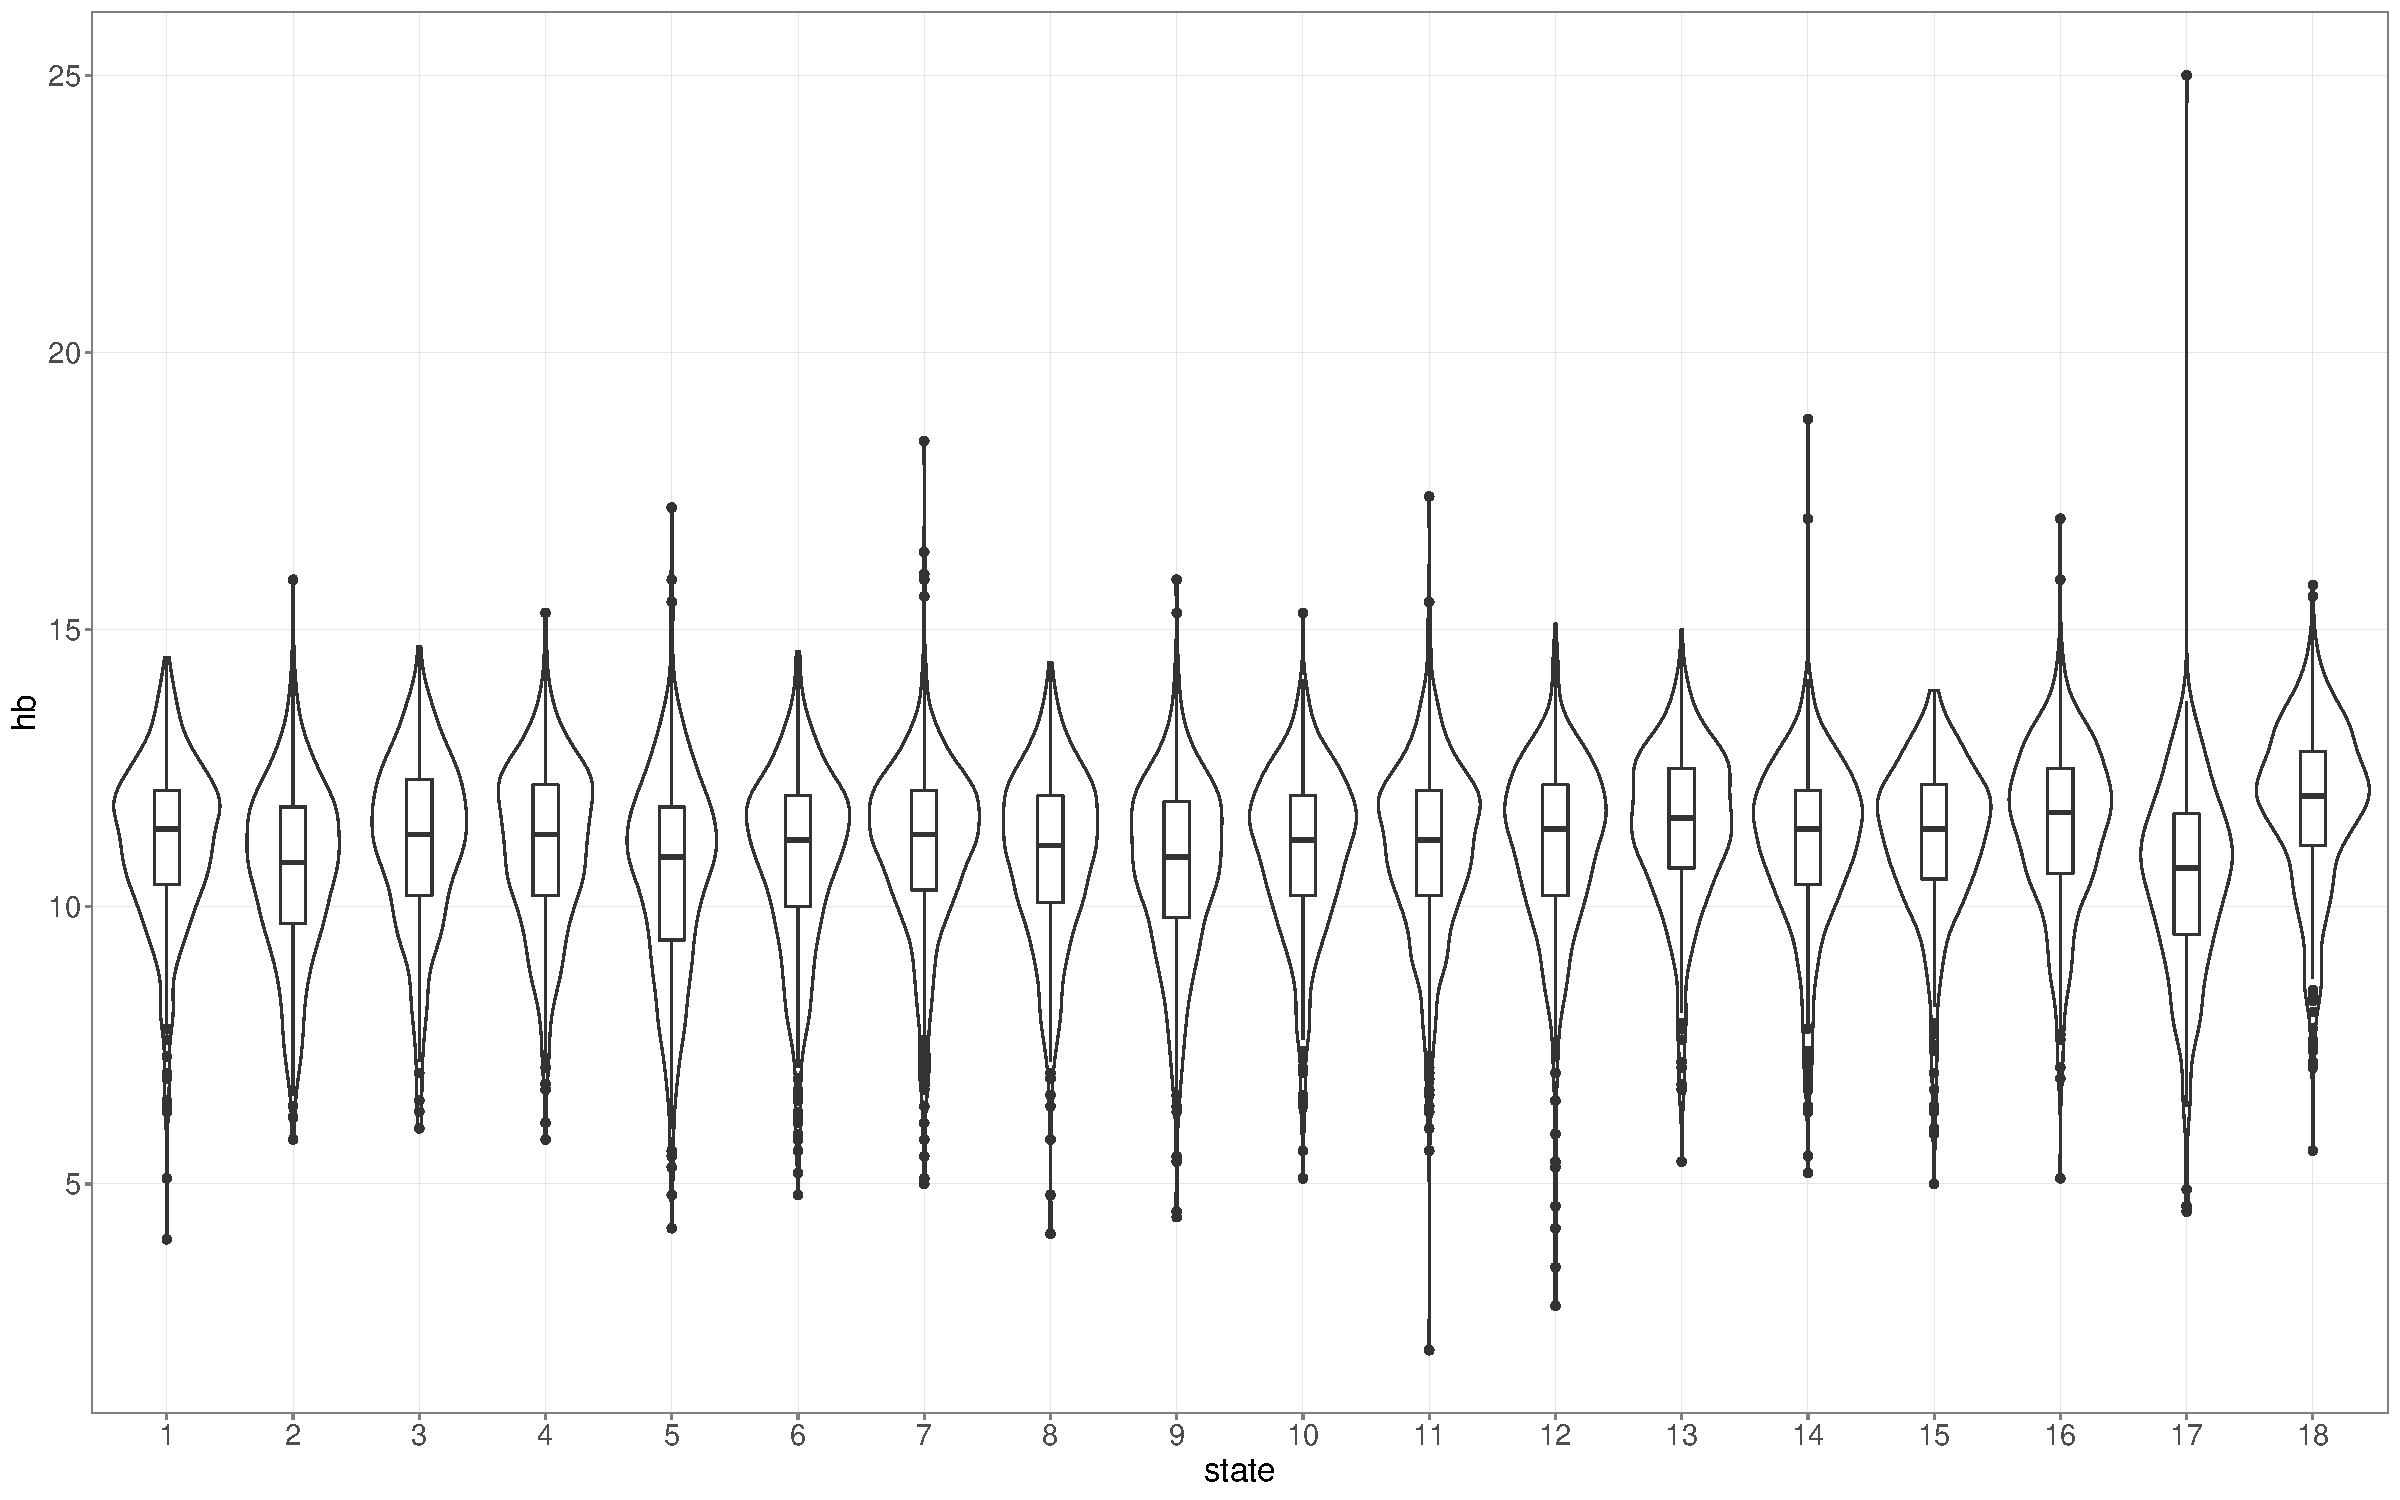
\includegraphics{sudanMNindicators_files/figure-latex/violin-1} 

}

\caption{Example violin plot for Hb in children 6-59 months sample by state}\label{fig:violin}
\end{figure}

For absurdly high or low outliers such as that in State 17, we propose to winsorize with the aim of discarding as little data as possible by brining down high values or bringing up low values enough that no bias is introduced into the estimate of mean values.

\newpage

\renewcommand\refname{References}
\bibliography{micronutrient.bib}

\end{document}
